\documentclass[letterpaper,11pt]{memoir}
  \usepackage[utf8]{inputenc}
  \renewcommand{\sfdefault}{Myriad-LF} % titres en MyriadPro
  \usepackage[english,francais]{babel}
  \usepackage[absolute]{textpos}
  \usepackage{graphicx,amsmath,vgmath,fourier}

\begin{document}

\frontmatter

\pagestyle{empty}

\textblockorigin{0mm}{0mm}
\setlength{\parindent}{0mm}

\begin{textblock*}{216mm}(0mm,0mm)
  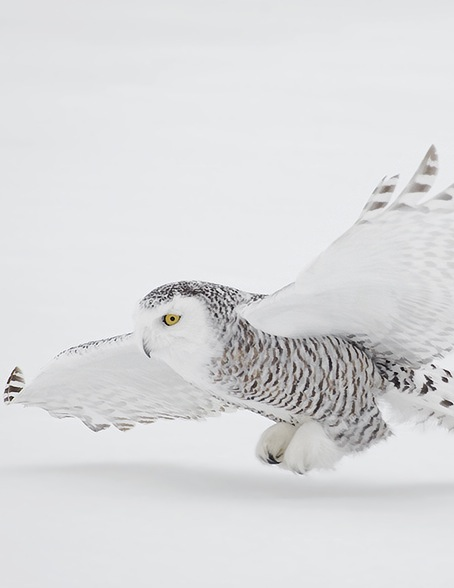
\includegraphics[height=11in,keepaspectratio=true]{harfang.jpg} \\
\end{textblock*}

\begin{textblock*}{176mm}(20mm,30mm)
  \sffamily
  \fontseries{b}\fontsize{42}{42}\selectfont
  \rule{\linewidth}{0.5pt}
  Introduction à la \\
  programmation en R \\[-19pt]
  \rule{\linewidth}{0.5pt}
\end{textblock*}

\begin{textblock*}{176mm}(20mm,80mm)
  \sffamily
  \fontseries{m}\fontsize{24}{24}\selectfont
  Vincent Goulet
\end{textblock*}

\mbox{}
% \begin{adjustwidth*}{-14.2mm}{-30mm}
%   \sffamily
%   \raggedright
%   \vspace*{-15mm}
%   \fontseries{b}\fontsize{42}{42}\selectfont
%   Introduction à la \\
%   programmation en R \\[-12pt]
%   \vspace*{32mm}
%   \fontseries{m}\fontsize{24}{36}\selectfont
%   Vincent Goulet
% \end{adjustwidth*}

\newpage

\begin{textblock*}{93mm}[1,0](216mm,0mm)
  
\includegraphics[height=11in,keepaspectratio=true]{harfang-arriere.jpg} \\
\end{textblock*}

\begin{textblock*}{123mm}[0,0](10mm,240mm)
  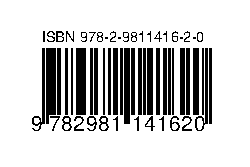
\includegraphics[keepaspectratio=true]{codebarre} \\
\end{textblock*}

\end{document}

%%% Local Variables:
%%% mode: latex
%%% TeX-master: t
%%% End:
